% --------------------------------------------------
% APPENDIX
% --------------------------------------------------
\appendix
\section{Supplementary Tables and Figures}
\label{sec:appendix}

\begin{table}[H]
\centering
\caption{Variable definitions and economic interpretations.}
\label{tab:variables}
\small
\renewcommand{\arraystretch}{1.3}
\begin{tabular}{@{} p{2.6cm} p{11cm} @{}}
\toprule
\textbf{Variable} & \textbf{Definition and interpretation} \\
\midrule
GC contender      & =1 if top-20 GC finish in any Grand Tour in the prior two years. \textit{Tournament incentives: higher expected returns from continuation.} \\
Prev.\ DNF rate   & Share of prior starts ending in abandonment. \textit{Revealed risk type and continuation cost.} \\
Age               & Rider's age at race start. \textit{Human capital: maturity and decline.} \\
Experience        & Grand Tours started prior to current race. \textit{Human capital: knowledge and durability.} \\
Tour de France    & =1 for TdF (Vuelta as baseline). \textit{Highest media, sponsor, and UCI point value.} \\
Giro d'Italia     & =1 for Giro. \textit{Intermediate event prestige.} \\
Mountain stage    & =1 if mountain stage (time-varying). \textit{Highest marginal cost of effort.} \\
Distance (z)      & Standardised stage distance (time-varying). \textit{Physically more taxing stages.} \\
Team size         & Riders on team at race start (7--9). \textit{Team-resource control.} \\
Team avg.\ age    & Mean age of starting team riders. \textit{Team-resource control.} \\
Year (centred)    & Calendar year minus sample mean. \textit{Secular abandonment trend.} \\
\bottomrule
\end{tabular}
\end{table}

\begin{table}[H]
\centering
\caption{Cox PH model estimated on GC contenders only. The previous DNF rate effect is substantially larger than in the pooled model, consistent with higher stakes for riders whose abandonment carries a stronger career signal.}
\label{tab:cox_gc}
\small
\renewcommand{\arraystretch}{1.3}
\begin{tabular}{@{} lrrrr @{}}
\toprule
Variable & Hazard Ratio & 95\% CI & $p$-value & \\
\midrule
Age                 & 1.007 & [0.980, 1.036] & 0.599 & \\
Experience          & 1.008 & [0.983, 1.035] & 0.520 & \\
Previous DNF rate   & 2.280 & [1.379, 3.771] & 0.001 & ** \\
Team size           & 1.134 & [0.896, 1.436] & 0.296 & \\
Team average age    & 1.033 & [0.970, 1.100] & 0.310 & \\
Tour de France      & 0.863 & [0.696, 1.069] & 0.177 & \\
Giro d'Italia       & 1.195 & [0.961, 1.486] & 0.110 & \\
Year (centred)      & 0.995 & [0.968, 1.022] & 0.708 & \\
\bottomrule
\multicolumn{5}{l}{\footnotesize ** $p<0.01$. Baseline race: Vuelta a Espa\~{n}a. $N = 1{,}395$.}
\end{tabular}
\end{table}

\begin{table}[H]
\centering
\caption{Cox PH model estimated on non-GC riders only. The Tour de France protective effect is significant in this sub-sample but not for GC contenders, suggesting that event-value incentives operate mainly through domestiques and support riders.}
\label{tab:cox_nonGC}
\small
\renewcommand{\arraystretch}{1.3}
\begin{tabular}{@{} lrrrr @{}}
\toprule
Variable & Hazard Ratio & 95\% CI & $p$-value & \\
\midrule
Age                 & 0.996 & [0.985, 1.008] & 0.533 & \\
Experience          & 1.003 & [0.991, 1.014] & 0.634 & \\
Previous DNF rate   & 1.472 & [1.238, 1.750] & $<$0.001 & *** \\
Team size           & 0.967 & [0.872, 1.071] & 0.518 & \\
Team average age    & 0.978 & [0.953, 1.004] & 0.103 & \\
Tour de France      & 0.866 & [0.784, 0.957] & 0.005 & ** \\
Giro d'Italia       & 1.041 & [0.948, 1.144] & 0.398 & \\
Year (centred)      & 0.999 & [0.988, 1.011] & 0.915 & \\
\bottomrule
\multicolumn{5}{l}{\footnotesize *** $p<0.001$, ** $p<0.01$. Baseline race: Vuelta a Espa\~{n}a. $N = 7{,}650$.}
\end{tabular}
\end{table}

\begin{table}[H]
\centering
\caption{Schoenfeld residual test of the proportional hazards assumption. No covariate is significant at the 5\% level, indicating that the proportional hazards assumption is not rejected for any variable.}
\label{tab:schoenfeld}
\small
\renewcommand{\arraystretch}{1.3}
\begin{tabular}{@{} lrr @{}}
\toprule
Variable & Test statistic & $p$-value \\
\midrule
Age                 & 0.865 & 0.352 \\
Experience          & 0.242 & 0.623 \\
Previous DNF rate   & 0.034 & 0.854 \\
GC contender        & 0.078 & 0.780 \\
Team size           & 0.575 & 0.448 \\
Team average age    & 1.904 & 0.168 \\
Tour de France      & 0.871 & 0.351 \\
Giro d'Italia       & 1.075 & 0.300 \\
Year (centred)      & 0.638 & 0.424 \\
\bottomrule
\end{tabular}
\end{table}

\begin{figure}[H]
    \centering
    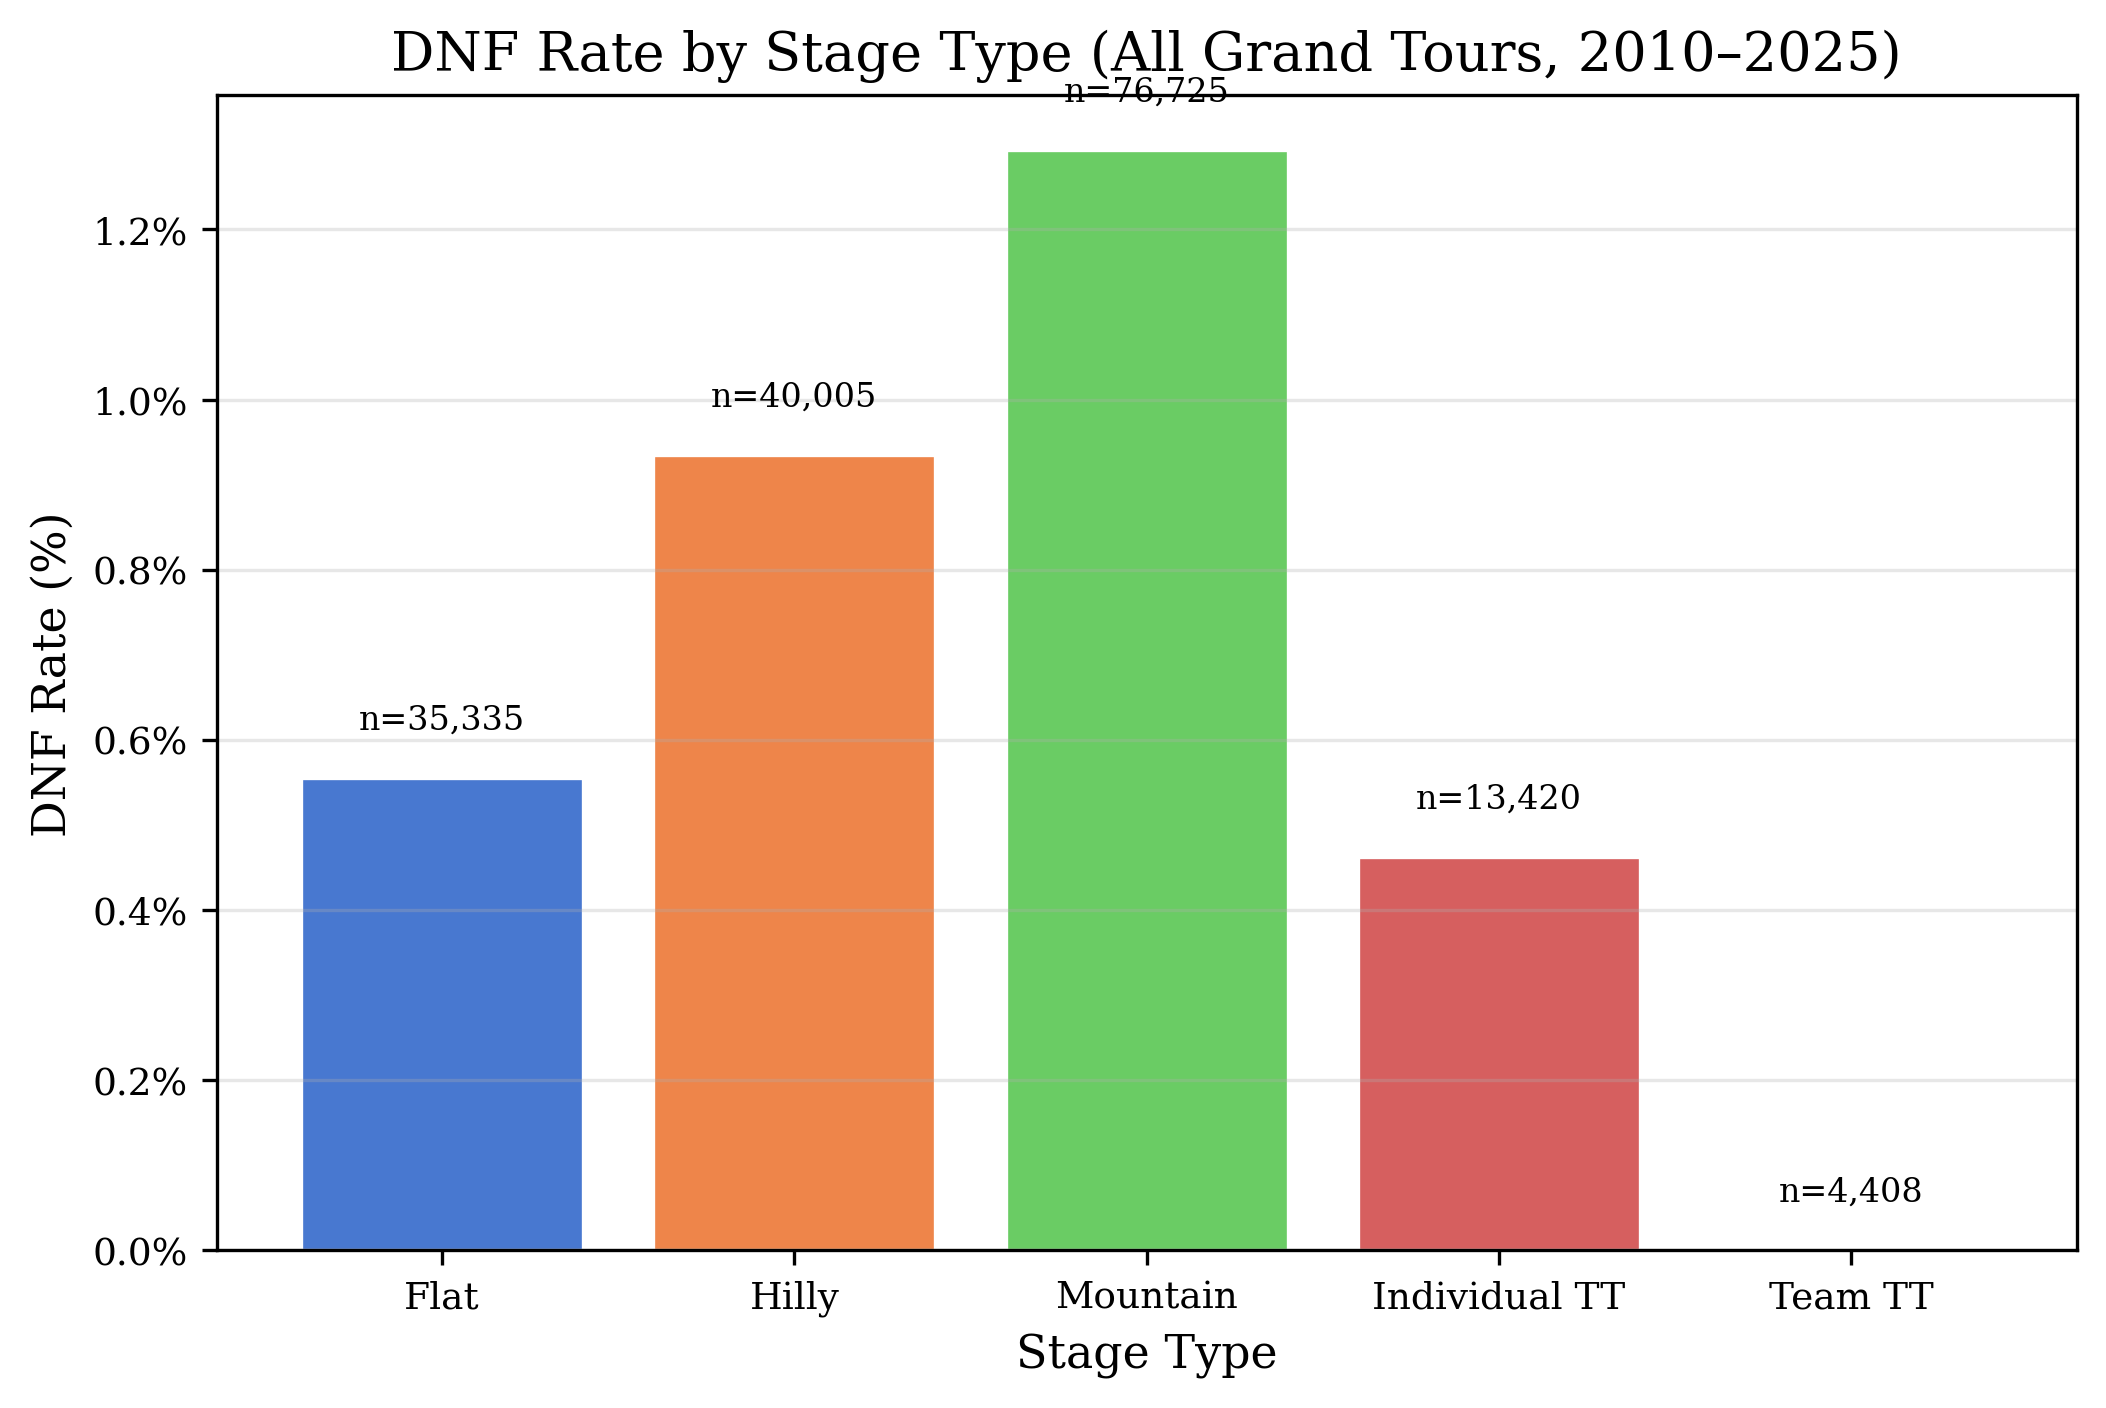
\includegraphics[width=0.70\linewidth]{Afsnit/Billeder/fig3_dnf_rate_by_stage_type.png}
    \caption{DNF rate by stage type across all Grand Tours and editions (2010--2025). Mountain stages show the highest abandonment rates, consistent with the time-varying Cox model result that mountain stages raise daily abandonment hazard.}
    \label{fig:dnf_by_stage_type}
\end{figure}

\begin{figure}[H]
    \centering
    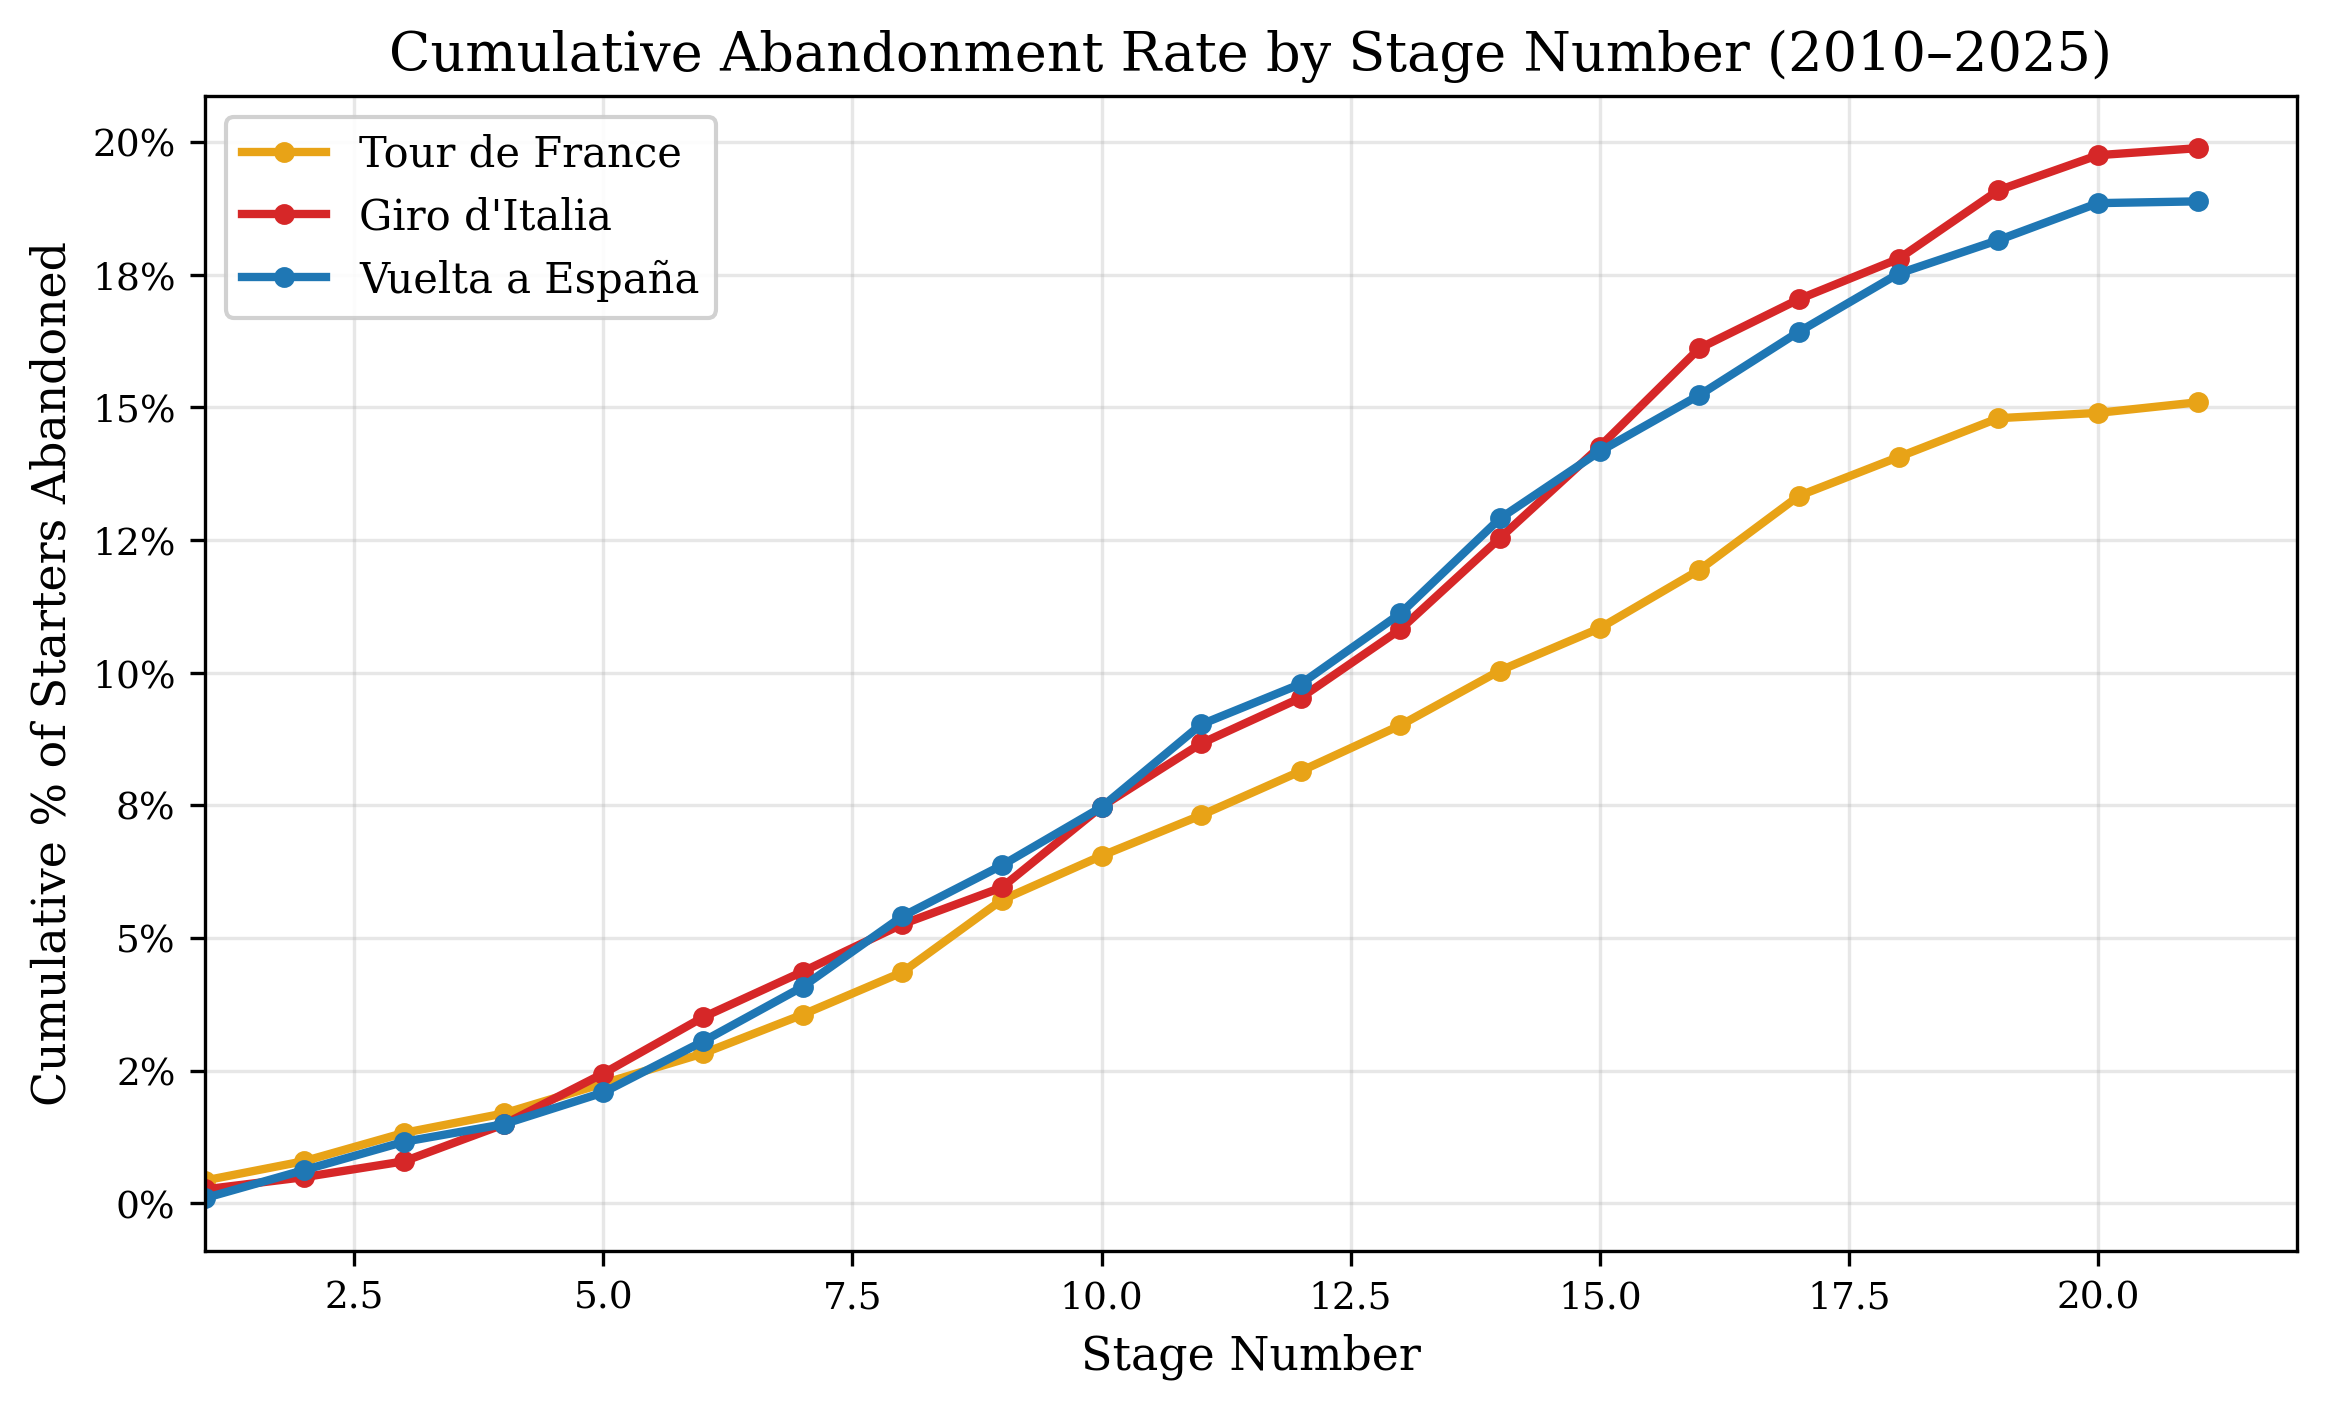
\includegraphics[width=0.70\linewidth]{Afsnit/Billeder/fig4_cumulative_dnf_by_stage.png}
    \caption{Cumulative DNF rate by stage number, averaged across all Grand Tour editions. The roughly linear accumulation of abandonments across stages is consistent with a relatively constant per-stage hazard, with no sharp spike at any particular stage.}
    \label{fig:cumulative_dnf}
\end{figure}

\begin{figure}[H]
    \centering
    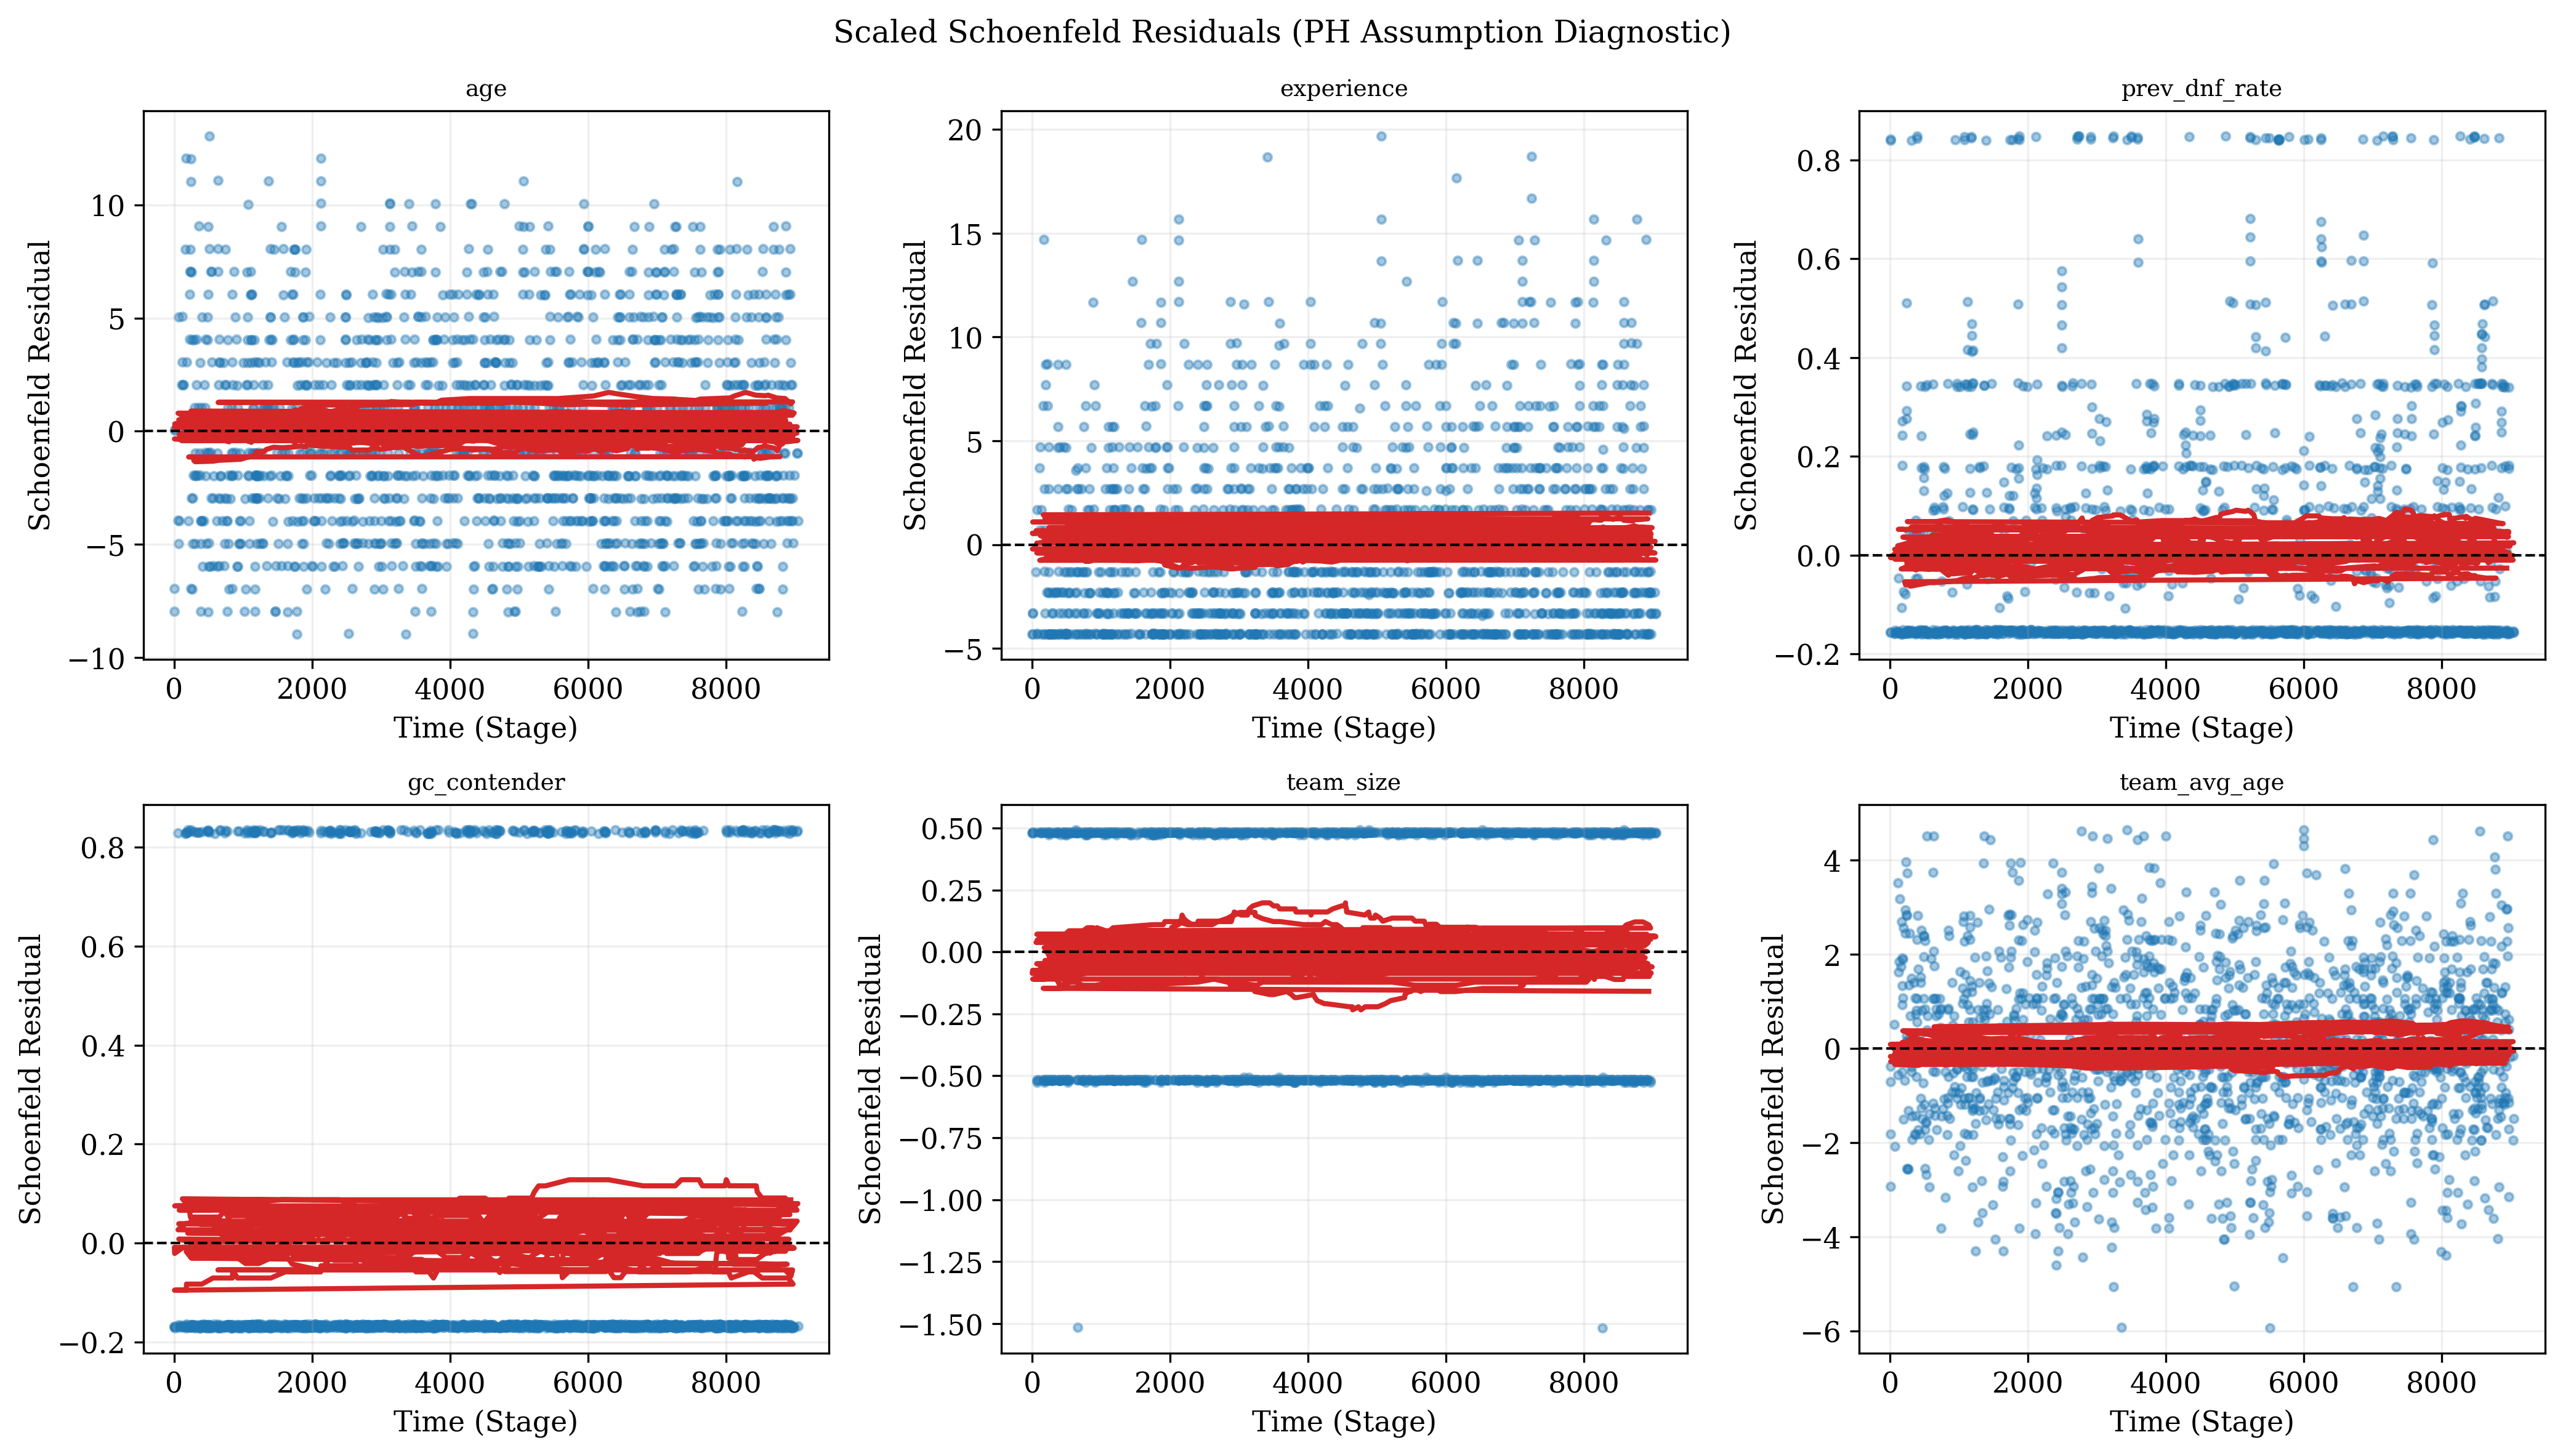
\includegraphics[width=0.90\linewidth]{Afsnit/Billeder/fig6_schoenfeld_residuals.png}
    \caption{Schoenfeld residual plots for each covariate in the basic Cox PH model. Under the null hypothesis of proportional hazards, the residuals should show no systematic trend over time. No covariate exhibits a clear trend, providing visual confirmation of the formal test results reported in Table~\ref{tab:schoenfeld}.}
    \label{fig:schoenfeld}
\end{figure}
